\documentclass{article}
\usepackage[paperwidth=650pt,paperheight=385pt,margin=0pt]{geometry}
\usepackage{fontspec}
\setmainfont{SourceSans3-Regular.otf}
\usepackage{tikz}
\usetikzlibrary{arrows.meta}
\pagestyle{empty}
\definecolor{tinta}{HTML}{17394A}
\definecolor{azul}{HTML}{EAF1F6}
\definecolor{verde}{HTML}{EAF4EE}
\definecolor{borde}{HTML}{9CB1BC}
\begin{document}
\noindent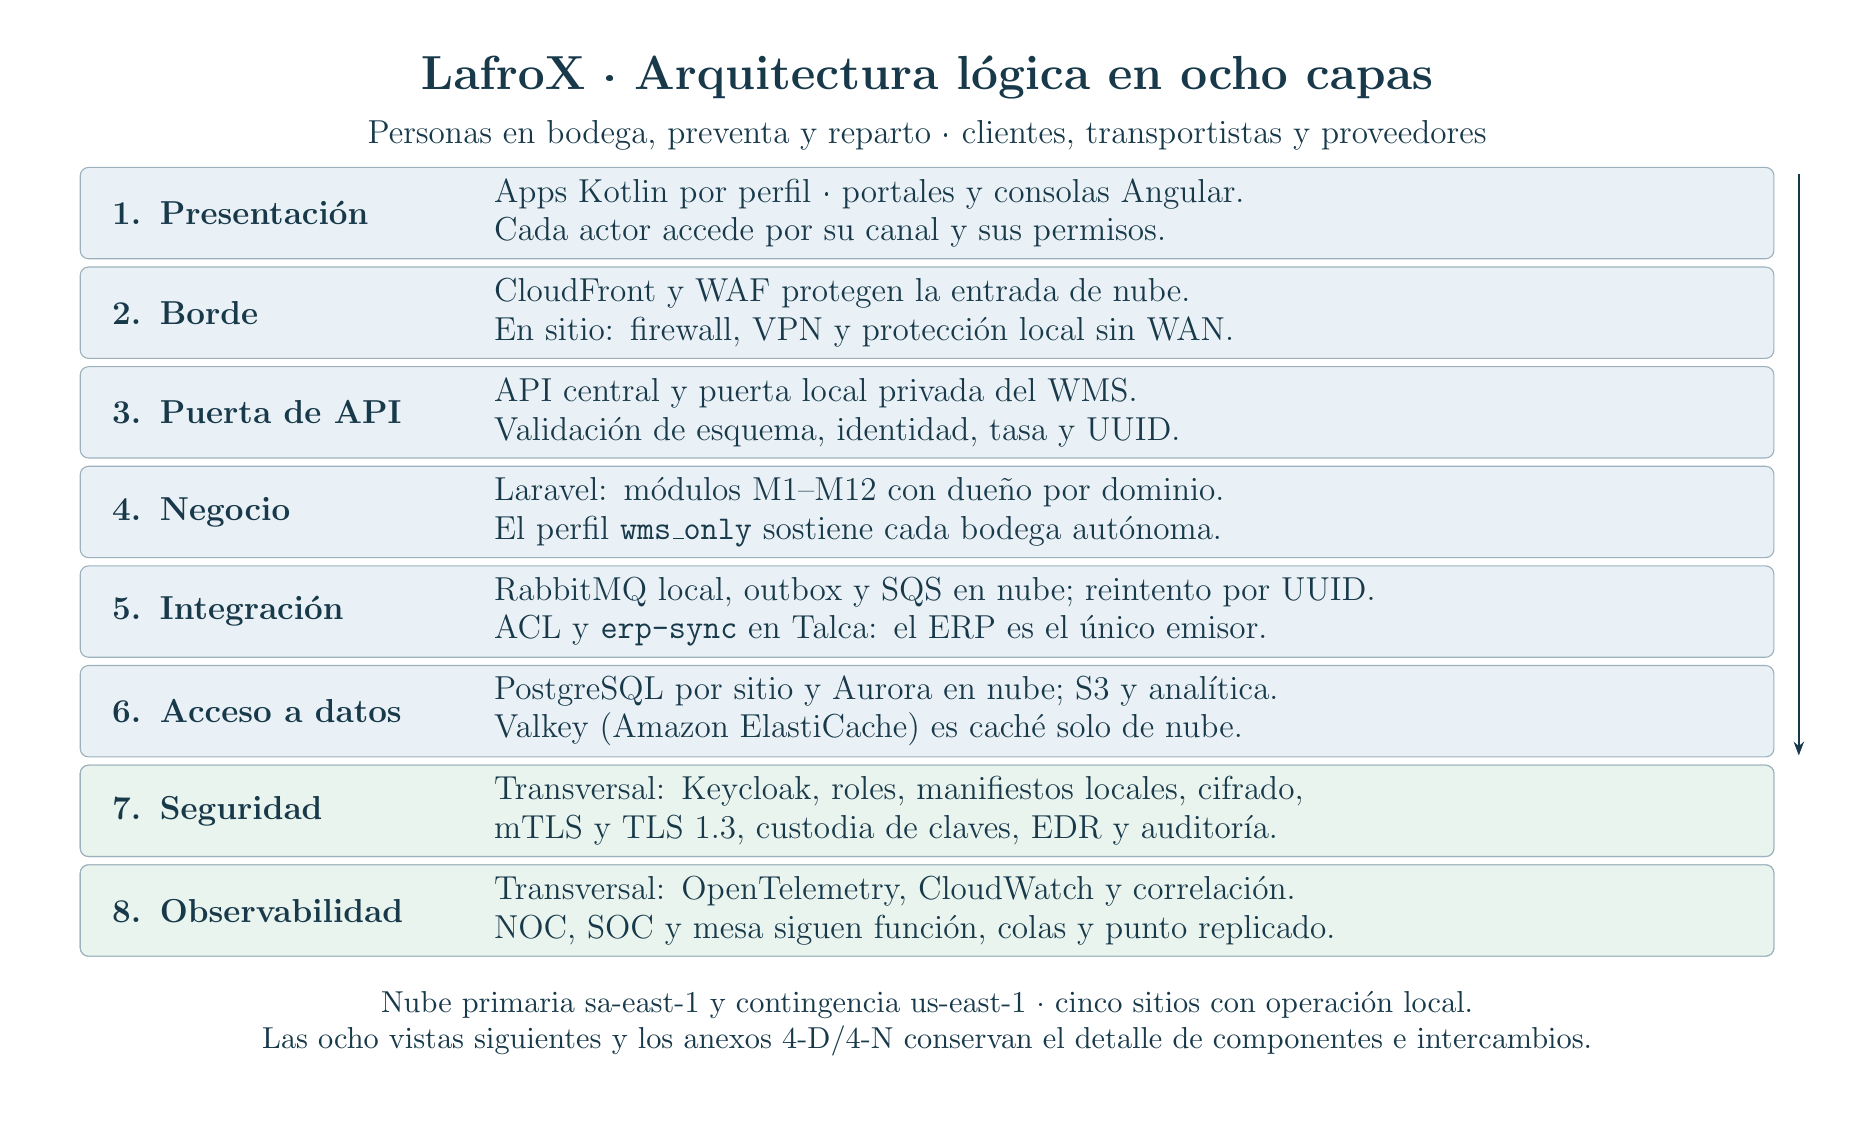
\begin{tikzpicture}[x=1pt,y=1pt,
  capa/.style={draw=borde,rounded corners=3pt,fill=azul,
    minimum width=612pt,minimum height=33pt,inner sep=0pt},
  nombre/.style={anchor=west,text=tinta,font=\bfseries\fontsize{12pt}{14pt}\selectfont,text width=134pt},
  detalle/.style={anchor=west,text=tinta,font=\fontsize{12pt}{14pt}\selectfont,text width=454pt,align=left}]
\path[use as bounding box] (0,0) rectangle (650,385);
\node[text=tinta,font=\bfseries\fontsize{16pt}{19pt}\selectfont] at (325,367) {LafroX · Arquitectura lógica en ocho capas};
\node[text=tinta,font=\fontsize{12pt}{14pt}\selectfont] at (325,346) {Personas en bodega, preventa y reparto · clientes, transportistas y proveedores};
\foreach \y in {318,282,246,210,174,138,102,66} {\node[capa] at (325,\y) {};}
\node[nombre] at (27,318) {1. Presentación};
\node[detalle] at (165,318) {Apps Kotlin por perfil · portales y consolas Angular.\\Cada actor accede por su canal y sus permisos.};
\node[nombre] at (27,282) {2. Borde};
\node[detalle] at (165,282) {CloudFront y WAF protegen la entrada de nube.\\En sitio: firewall, VPN y protección local sin WAN.};
\node[nombre] at (27,246) {3. Puerta de API};
\node[detalle] at (165,246) {API central y puerta local privada del WMS.\\Validación de esquema, identidad, tasa y UUID.};
\node[nombre] at (27,210) {4. Negocio};
\node[detalle] at (165,210) {Laravel: módulos M1--M12 con dueño por dominio.\\El perfil \texttt{wms\_only} sostiene cada bodega autónoma.};
\node[nombre] at (27,174) {5. Integración};
\node[detalle] at (165,174) {RabbitMQ local, outbox y SQS en nube; reintento por UUID.\\ACL y \texttt{erp-sync} en Talca: el ERP es el único emisor.};
\node[nombre] at (27,138) {6. Acceso a datos};
\node[detalle] at (165,138) {PostgreSQL por sitio y Aurora en nube; S3 y analítica.\\Valkey (Amazon ElastiCache) es caché solo de nube.};
\node[capa,fill=verde] at (325,102) {};
\node[nombre] at (27,102) {7. Seguridad};
\node[detalle] at (165,102) {Transversal: Keycloak, roles, manifiestos locales, cifrado,\\mTLS y TLS 1.3, custodia de claves, EDR y auditoría.};
\node[capa,fill=verde] at (325,66) {};
\node[nombre] at (27,66) {8. Observabilidad};
\node[detalle] at (165,66) {Transversal: OpenTelemetry, CloudWatch y correlación.\\NOC, SOC y mesa siguen función, colas y punto replicado.};
\draw[-{Stealth[length=5pt]},tinta,line width=.8pt] (640,332)--(640,122);
\node[text=tinta,font=\fontsize{11pt}{13pt}\selectfont,align=center] at (325,25)
 {Nube primaria sa-east-1 y contingencia us-east-1 · cinco sitios con operación local.\\Las ocho vistas siguientes y los anexos 4-D/4-N conservan el detalle de componentes e intercambios.};
\end{tikzpicture}
\end{document}
